Automatic differentiation (AD) is a technology that allows computing gradients thought a computer program. The main idea is that every computer program manipulating numbers can be reduced to a sequence of simple algebraic operations that can be easily differentiable. The derivatives of the outputs of the computer program with respect to their inputs are then combined using the chain rule.
One advantage of AD systems is that we can automatically differentiate programs that include control flow, such as branching, loops or recursions. This is because at the end of the day, any program can be reduced to a trace of input, intermediate and output variables \cite{Baydin_Pearlmutter_Radul_Siskind_2015}.

Sometimes AD is compared against symbolic differentiation.
According to \cite{Laue2020}, these two are the same and the only difference is in the data structures used to implement them, while \cite{Elliott_2018} suggests that AD is symbolic differentiation performed by a compiler.

Depending if the concatenation of these gradients is done as we execute the program (from input to output) or in a later instance were we trace-back the calculation from the end (from output to input), we are going to talk about \textit{forward} or \textit{backward} AD, respectively.

Forward mode AD can be implemented in different ways depending on the data structures we use at the moment of representing a computer program. Examples of these data structures include dual numbers and Wengert lists (see \cite{Baydin_Pearlmutter_Radul_Siskind_2015} for a good review on these methods). Let's consider the case of dual numbers.
We can define an abstract type, defined as a dual number, composed of two elements:
\begin{equation}
 x_\epsilon = x_1 + \epsilon x_2,
\end{equation}
where $\epsilon$ is an abstract number with the property $\epsilon^2 = 0$ and $\epsilon \neq 0$.
Given two dual numbers $x_\epsilon = x_1 + \epsilon x_2$ and $y_\epsilon = y_1 + \epsilon y_2$, it is easy to derive using the fact $\epsilon^2=0$ that
\begin{equation}
 x_\epsilon y_\epsilon = x_1 y_1 + \epsilon(x_1 y_2 + x_2 y_1) \qquad
 \frac{x_\epsilon}{y_\epsilon} = \frac{x_1}{y_1} + \epsilon \frac{x_2 y_1 - x_1 y_2}{y_1^2}.
\end{equation}
From these last examples, we can see that the dual component of the dual number carries the information of the derivatives when combining operations.
Intuitively, we can think about $\epsilon$ as being a differential in the Taylor expansion:
\begin{equation}
 f(x + \epsilon) = f(x) + \epsilon f'(x) + \mathcal O (\epsilon^2)
\end{equation}
When computing first order derivatives, we can ignore everything of order $\epsilon^2$ or larger, which is represented in the condition $\epsilon^2 = 0$.
This implies that we can use dual numbers to implement forward AD through a numerical algorithm. Implementing such a type in a programming language implies defining what it means to perform basic operations and then combine them using the chain rule provided by the dual number properties.\footnote{See \url{https://alemorales.info/post/automatic-differentiation-with-dual-numbers/} for an example on how these operations can be implemented in Julia.}

Backward mode AD is also known as the adjoint of cotangent linear mode, or backpropagation in the field of machine learning. Given a directional graph of operations defined by a Wengert list, we can compute gradients of any given function backwards as
\begin{equation}
    \bar v = \frac{\partial \ell}{\partial v_i}= \sum_{w : v \rightarrow w \in G} \frac{\partial w}{\partial v} \bar{w}.
\end{equation}

Another way of implementing backwards AD is by defining a \textit{pullback} function \cite{Innes_2018}, a method also known as \textit{continuation-passing style} \cite{Wang_Zheng_Decker_Wu_Essertel_Rompf_2019}. In the backward step, this executes a series of functions calls, one for each elementary operation.
If one of the nodes in the graph $w$ is the output of an operation involving the nodes $v_1, \ldots, v_m$, where $v_i \rightarrow w$ are all nodes in the graph, then the pullback $\bar v_1, \ldots, \bar v_m = \mathcal B_w(\bar w)$ is a function that accepts gradients with respect to $w$ (defined as $\bar w$) and returns gradients with respect to each $v_i$ ($\bar v_i$) by applying the chain rule. Consider the example of the multiplicative operation $w = v_1 \times v_2$. Then
\begin{equation}
 \bar v_1, \bar v_2 = v_2 \times \bar w , \quad
 v_1 \times \bar w = \mathcal{B}_w (\bar w),
\end{equation}
which is equivalent to using the chain rule as 
\begin{equation}
 \frac{\partial \ell}{\partial v_1} = \frac{\partial}{\partial v_1}(v_1 \times v_2) \frac{\partial \ell}{\partial w}.
\end{equation}

In the Julia ecosystem, \texttt{ForwardDiff.jl} implements forward mode AD with multidimensional dual numbers \cite{RevelsLubinPapamarkou2016},
while \texttt{ReverseDiff.jl} and \texttt{Zygote.jl} use callbacks to compute gradients. When gradients are being computed with less than $\sim 100$ parameters, the former is faster (see documentation).

\subsection{AD connection with JVPs and VJPs}

When working with unit operations that involve matrix operations dealing with vectors of different dimensions, the order in which we apply the chain rule matters. When computing a gradient using AD, we can encounter vector-Jacobian products (VJPs) or Jacobian-vector products (JVP). As their name indicate, the difference between them regards the fact if the quantity we are interested in computing is described by the product of a Jacobian (the two dimensional matrix with the gradients as rows) by a vector on the left
side (VJP) or the right (JVP).

For the examples we care here, the Jacobian is described as the product of multiple Jacobian using the chain rule. In this case, the full gradient is computed as the chain product of vectors and Jacobians. Let's consider for example the case of a loss function $L : \mathbb R^n \mapsto \mathbb R$ that can be decomposed as $L(\theta) = \ell \circ g_{k} \circ \ldots \circ g_2 \circ g_1(\theta)$, with $\ell : \mathbb R^{d_k} \mapsto \mathbb R$ the final evaluation of the loss function after we apply in order a sequence of intermediate functions $g_i : \mathbb R^{d_{i-1}} \mapsto \mathbb R^{d_i}$, $d_0 = n$. Examples of this are neural networks and iterative differential equation solvers. Now, using the chain rule, we can calculate the gradient of the final loss funcition as
\begin{equation}
 \nabla_\theta L = \nabla \ell \cdot Dg_{k} \cdot Dg_{k-1} \cdot \ldots \cdot Dg_2 \cdot Dg_1.
\end{equation}
Notice that in the last equation, $\nabla \ell \in \mathbb R^{d_k}$ is a vector, while all the other term $Dg_i$ are full matrices. In order to compute $\nabla_\theta L$, we can solve the multiplication starting from the right side, which will correspond to multiple the Jacobians forward in time from $Dg_1$ to $Dg_k$, or from the left side, moving backwards in time. The important aspect of this last case is that we will always been computing VJPs, since the product of a vector and a matrix is a vector. Since VJP are easier to evaluate than full Jacobians, the backward mode will be in general faster (see Figure \ref{fig:vjp-jvp}). For general rectangular matrices $A\in \mathbb R^{d_1 \times d_2}$ and $B \in \mathbb R^{d_2 \times d_3}$, the cost of the matrix multiplication $AB$ is $\mathcal O (d_1 d_2 d_3)$. This implies that forward AD requires a total of
\begin{equation}
 d_2 d_1 n + d_3 d_2 n + \ldots + d_k d_{k-1} n + d_k n = \mathcal O (kn)
\end{equation}
operations, while backwards mode AD requires
\begin{equation}
 d_k d_{k-1} + d_{k-1} d_{k-2} + \ldots + d_2 d_1 + d_1 n = \mathcal O (k + n)
\end{equation}
operations.
In general, when the function we are trying to differentiate has a larger input space than output, which is usually the case when working with scalar loss functions, AD in backward mode is more efficient as it propagates the chain rule by computing VJPs. On the other side, when the output dimension is larger than the input space dimension, forwards AD is more efficient. This is the reason why in most machine learning application people use backwards AD. However, notice that backwards mode AD requires us to save the solution thought the forward run in order to run backwards afterwards, while in forward mode we can just evaluate the gradient as we iterate our sequence of functions. This means that for problems with a small number of parameters, forward mode can be faster and more memory-efficient that backwards AD.

\begin{figure}
    \centering
    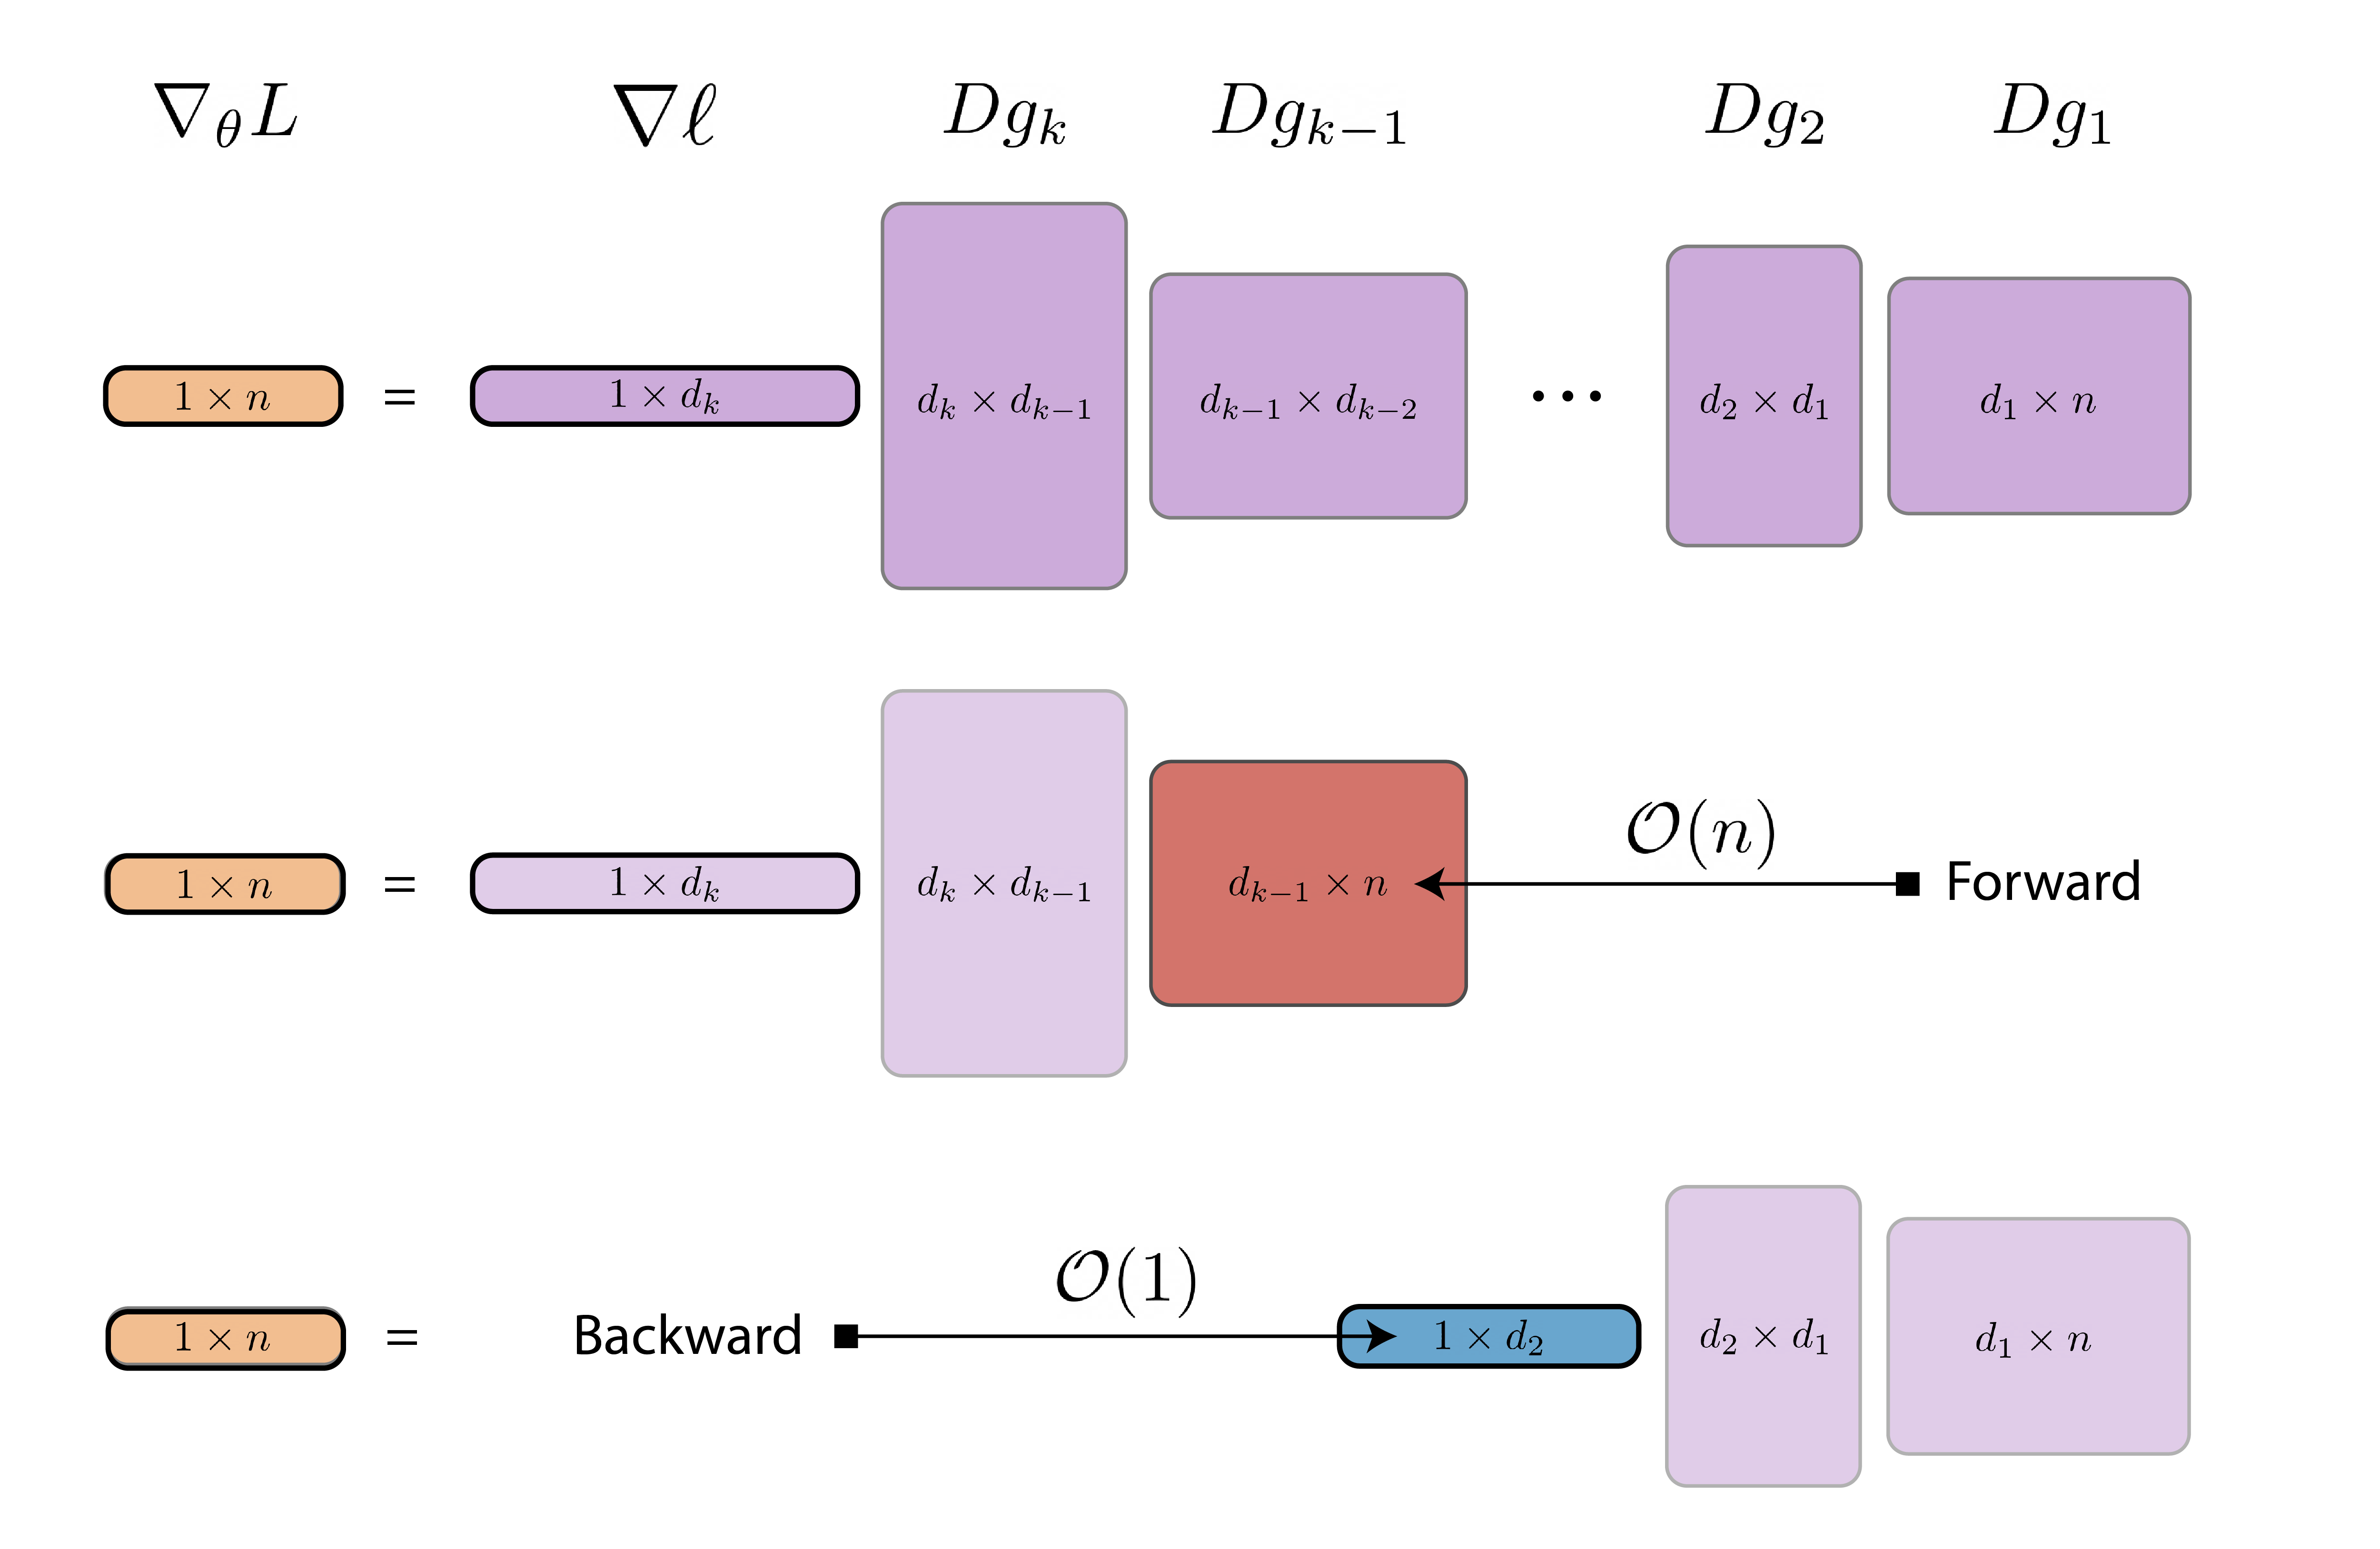
\includegraphics[width=0.95\textwidth]{figures/VJP-JVP.png}
    \caption{Comparison between forward and backward AD.}
    \label{fig:vjp-jvp}
\end{figure}